\documentclass[11pt, a4paper]{article}
\usepackage[utf8]{inputenc}
\usepackage[T1]{fontenc}
\usepackage{lmodern}
\usepackage{amsmath}
\usepackage{graphicx}
\usepackage{csquotes}
\usepackage[style=apa,backend=biber]{biblatex}
\usepackage{titling}
\usepackage{setspace}
\onehalfspacing
\setlength{\droptitle}{-4em}
\addbibresource{references.bib}
\graphicspath{ {./Drawings/} }

\begin{document}
\author{Carlos Sebastian Madrigal Rodriguez}
\title{
    \textbf{Impacto de las Bases de Datos Vectoriales en la Recuperación de Información para Agentes de IA Especializados en Documentación de API SDN}
}
\date{\today}

\maketitle

% ==================== Introducción ====================

\section{Introducción}
\label{sec:introduction} 

Las redes modernas definidas por software (SDN) exponen numerosas APIs para configuración, monitoreo y gestión operativa. Sin embargo, el volumen y la complejidad de la documentación técnica dificultan que los ingenieros y sistemas de automatización identifiquen eficientemente las APIs apropiadas.

Las arquitecturas de Generación Aumentada por Recuperación (RAG, por sus siglas en inglés) ofrecen un enfoque prometedor para este desafío al combinar grandes modelos de lenguaje con fuentes de conocimiento externas. Mediante la recuperación semántica, estos sistemas pueden acceder y razonar sobre documentación técnica en tiempo real, permitiendo que los agentes de IA descubran APIs relevantes y apoyen flujos de trabajo de automatización más allá de la búsqueda tradicional basada en palabras clave \parencite{lewis2020rag,wu2024ragsurvey}.

Las bases de datos vectoriales constituyen un componente clave de las arquitecturas RAG al permitir búsquedas de similitud eficientes sobre representaciones vectoriales de la documentación. Esta capacidad puede mejorar el descubrimiento de información técnica relevante y facilitar el razonamiento contextual sobre grandes repositorios de APIs \parencite{johnson2019faiss}.

A pesar de su creciente adopción, la efectividad de las bases de datos vectoriales para la recuperación de documentación técnica en la automatización de redes sigue siendo insuficientemente comprendida. Por lo tanto, esta investigación examina el uso de bases de datos vectoriales para la recuperación impulsada por IA de documentación de API SDN y evalúa el rendimiento de bases de datos líderes en la industria como FAISS, PGVector y Neo4j en términos de precisión de recuperación, calidad de respuesta y rendimiento operativo.

% ==================== Materiales y Métodos ====================

\section{Materiales y Métodos}
\label{sec:Materials_and_Methods}
\subsection{Hipótesis}

\noindent\textbf{Hipótesis 1 (Principal):}
La incorporación de bases de datos vectoriales en agentes de IA basados en RAG mejora la recuperación de conocimiento y el descubrimiento de APIs en documentación SDN en comparación con los métodos de búsqueda tradicionales.

\noindent\textbf{Hipótesis 2:}
La recuperación basada en bases de datos vectoriales logra mayor precisión de recuperación que la búsqueda basada en palabras clave.

\noindent\textbf{Hipótesis 3:}
Las implementaciones de bases de datos vectoriales como FAISS, PGVector y Neo4j exhiben diferencias estadísticamente significativas en precisión de recuperación, calidad de respuesta y latencia.

\noindent\textbf{Hipótesis Nula:}
La elección de la base de datos vectorial no afecta significativamente la calidad de las respuestas generadas por los agentes de IA basados en RAG.\\

\subsection{Adquisición de Datos y Consideraciones Éticas}

El corpus experimental fue construido a partir de la documentación de API DevNet de Cisco SD-WAN disponible públicamente \parencite{cisco_sdwan_docs} y la especificación OpenAPI proporcionada por Cisco SD-WAN vManage \parencite{cisco_vmanage_openapi}.

El contenido se procesa únicamente para apoyar los experimentos de recuperación; los documentos originales permanecen como propiedad de sus respectivos dueños y no se redistribuyen. Todas las fuentes se referencian para garantizar transparencia y reproducibilidad.

\subsection{Reconocimiento y Preprocesamiento de Datos}
Los datos de API en formato JSON que proporciona la especificación OpenAPI de Cisco SD-WAN vManage \parencite{cisco_vmanage_openapi} se analizan para extraer los campos relevantes para la indexación y recuperación. Los principales campos extraídos se resumen en la Tabla \ref{tab:openapi-fields}.

\begin{table}[h]
    \centering
    \begin{tabular}{|l|p{9cm}|}
        \hline
        \textbf{Campo} & \textbf{Significado} \\
        \hline
        path & URL de la API \\
        \hline
        method & GET/POST/PUT/DELETE \\
        \hline
        tags & Categoría funcional \\
        \hline
        summary & Descripción breve \\
        \hline
        description & Descripción detallada \\
        \hline
        operationId & Nombre único de operación \\
        \hline
        parameters & Parámetros de entrada \\
        \hline
        requestBody & Carga útil de datos enviada\\
        \hline
        responses & Definición de salida \\
        \hline
    \end{tabular}
    \caption{Estructura principal de datos de la API.}
    \label{tab:openapi-fields}
\end{table}

Como tarea de preprocesamiento previa a la vectorización, los pares clave-valor se aíslan y convierten en cadenas de lenguaje natural. Por ejemplo, el endpoint de API para recuperar información de dispositivos podría transformarse en una cadena como la siguiente:

\begin{quote}
\textit{Ruta: Administration - Audit Log} \ \textit{Endpoint: GET /auditlog/page}\\
\textit{Operación: getStatBulkRawPropertyData}\\
\textit{Descripción: Obtener datos de propiedades en bruto de forma masiva.}\\
\textit{Parámetros: query (requerido), scrollId (opcional), count (requerido).}\\
\textit{Retorna: Datos del registro de auditoría.}
\end{quote}
\subsection{Tratamiento de Datos}
Los datos serán procesados a través de un pipeline (flujo sequencial) de ingestión común seguido de tres backends independientes de almacenamiento y recuperación. El pipeline de ingestión incluirá extracción de texto, limpieza y generación de representaciones vectoriales utilizando un modelo consistente (Qwen3-Embedding-4B, diseñado específicamente para tareas de incrustación y clasificación de texto) en todas las bases de datos para garantizar la comparabilidad. Cada base de datos se configurará siguiendo las mejores prácticas para un rendimiento y precisión de recuperación óptimos. La arquitectura general del pipeline de ingestión se ilustra en la Figura \ref{fig:ingestion_pipeline}.
\begin{figure}[h]
    \centering
    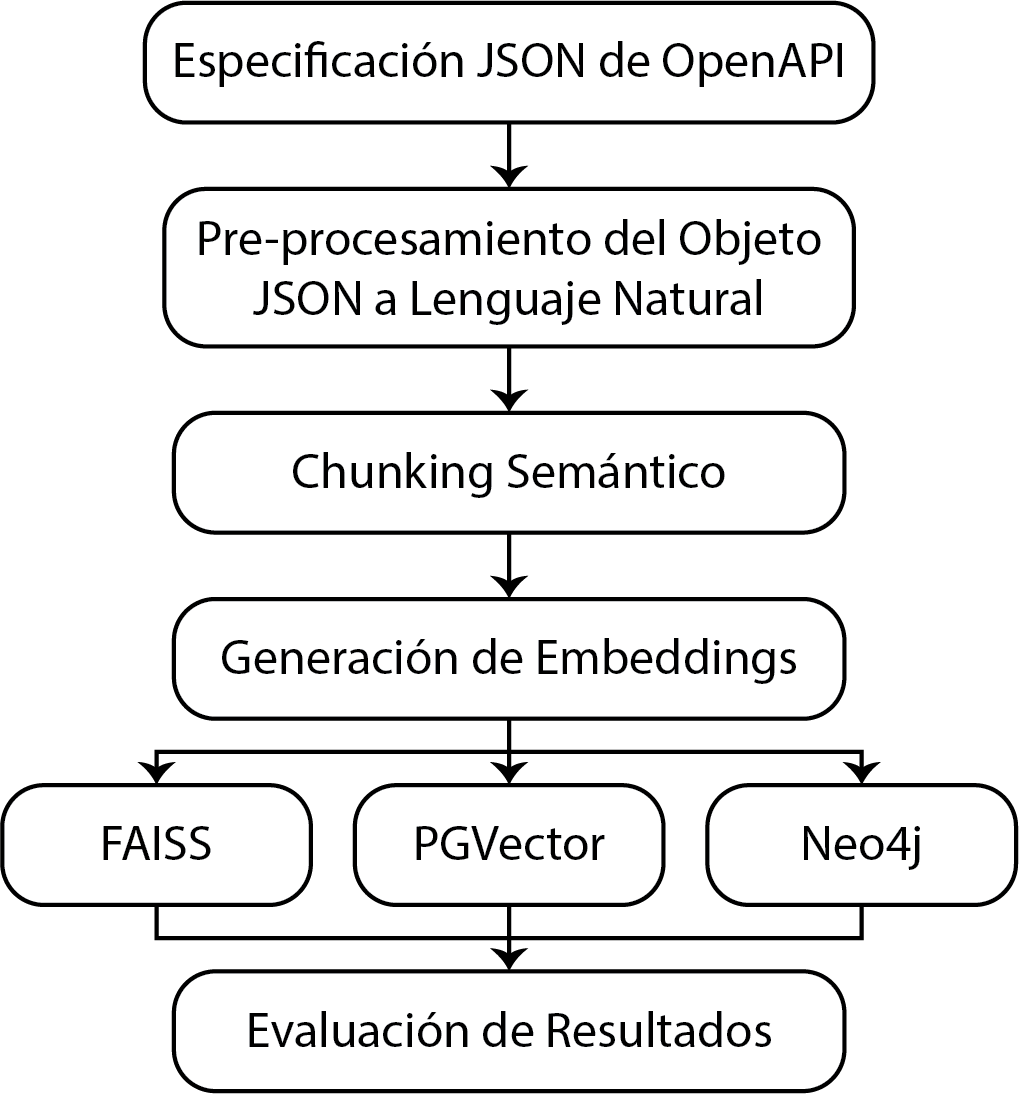
\includegraphics[width=0.45\textwidth]{Ingestion-Pipeline.png}
    \caption{Pipeline de ingestión para el procesamiento de datos de API.}
    \label{fig:ingestion_pipeline}
\end{figure}
    
\subsection{Métricas de Evaluación}
Los resultados de recuperación serán evaluados frente a un conjunto predefinido de consultas diseñadas para probar diversos aspectos del descubrimiento de APIs y la recuperación de información. Las consultas se subdividen en 3 grupos y se categorizan según su complejidad y relevancia para tareas típicas de automatización de redes:

\begin{itemize}
    \item \textbf{Grupo 1: Descubrimiento Básico de APIs}: Consultas que requieren identificar endpoints o parámetros de API específicos.
    \item \textbf{Grupo 2: Comprensión Contextual}: Consultas que requieren comprender el contexto del uso de la API, como dependencias o casos de uso comunes.
    \item \textbf{Grupo 3: Razonamiento Complejo}: Consultas que requieren razonamiento en múltiples pasos o síntesis de información a través de varias secciones de documentación.
\end{itemize}

Cada grupo contiene 15 consultas (45 en total). La precisión de recuperación se evaluará con cuatro métricas:

\begin{itemize}
    \item \textbf{Precisión@K}: Fracción de documentos relevantes en los K primeros resultados: $\frac{\text{relevantes en top-}K}{K}$
    \item \textbf{Recall@K}: Fracción de documentos relevantes recuperados sobre el total relevante: $\frac{\text{relevantes en top-}K}{\text{total relevantes}}$
    \item \textbf{MRR}: Promedio de los rangos recíprocos del primer documento relevante por consulta: $\frac{1}{|Q|} \sum_{i=1}^{|Q|} \frac{1}{\text{rank}_i}$
    \item \textbf{F1@K}: Media harmónica de Precisión@K y Recall@K: $2 \cdot \frac{P@K \cdot R@K}{P@K + R@K}$
\end{itemize}

La calidad de respuestas se evaluará con escala Likert y la latencia se medirá desde el envío de la consulta hasta la respuesta, con temporización automatizada.

\printbibliography[title={Referencias}]

\end{document}